\chapter{Case~Study: Fourth~Year~Project~System}

\todo{Fill this in}

\sectionnote {BM}
\section {Overview}

The fourth-year project management system is used by the department of Systems and Computer Engineering at Carleton University to manage the completion of fourth-year projects by students in software- and systems-related programs. The system is provides students with information on candidate projects, expectations, deadlines and deliverables, and also manages the submission of some project deliverables. The system is used by
\begin{itemize}
\item the \keyword{Project Coordinator}, who is an instructor responsible for overall administration of the fourth-year projects and events;
\item \keyword{Project Supervisors}, which are instructors who suggest candidate projects and supervise the completion of individual projects; and
\item \keyword{Project Group Members}, which are students who must be members of exactly one project group.
\end{itemize}

The system fulfills its functional requirements, but requires significant effort on the part of students to navigate, as all actions, information and deadlines are available at all times. It offers a good example of a system where the user experience could be improved by structuring the system into workflows. Additionally, the system involves deadlines and collaborative activities between multiple actors, which makes it a good test of the capabilities of the Stonepath workflow framework.

\sectionnote {BM}
\section {Requirements}
The required functionality of the fourth-year project management system can be split into three main concerns:
\begin{itemize}
\item \keyword{account management}, which involves creating accounts for Project Supervisors and Project Group Members, as well as authentication with the system;
\item \keyword{project selection}, which entails Project Supervisors creating candidate projects and managing group membership, as well as Project Group Members browsing available projects, consulting with Project Supervisors to find a project, and joining a project; and
\item \keyword{project execution}, which involves all of the collaboration between Project Group Members and the Project Supervisor(s) for their project.
\end{itemize}

Individual use cases for these concerns are illustrated in Figures \ref{fig:case-4ys-use-case-account-management} through \ref{fig:case-4ys-use-case-oral-reports}. Note that the project execution concern has been split into its own use case diagram (Figure \ref{fig:case-4ys-use-case-oral-reports}) as its requirements are somewhat more complex than the other phases of the project lifecycle.

\begin{figure}[!ht]
\centering 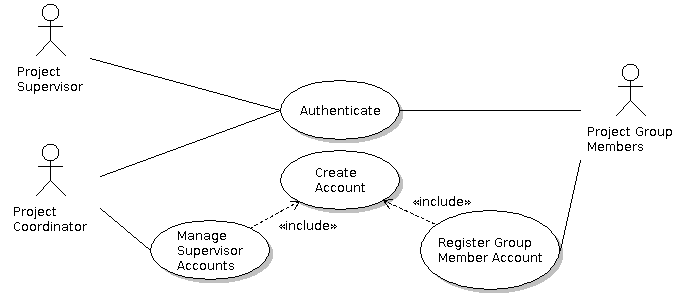
\includegraphics[width=6in]{./img/case-study-fourth-year-system/setup-and-provisioning}
\caption{Use case diagram for the account management functionality of the fourth-year project management system.}
\label{fig:case-4ys-use-case-account-management}
\end{figure}

\begin{figure}[!ht]
\centering 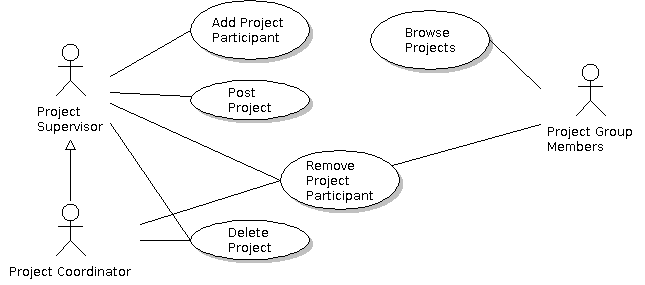
\includegraphics[width=6in]{./img/case-study-fourth-year-system/project-selection}
\caption{Use case diagram for the project selection functionality of the fourth-year project management system.}
\label{fig:case-4ys-use-case-project-selection}
\end{figure}

\begin{figure}[!ht]
\centering 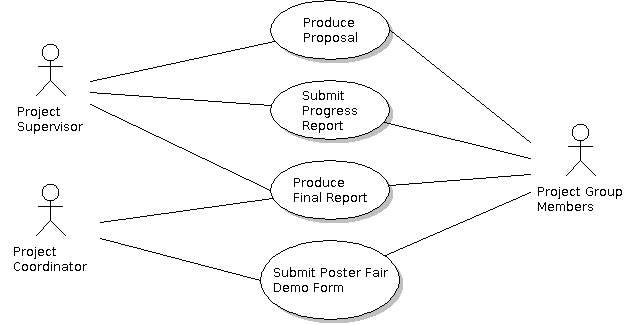
\includegraphics[width=6in]{./img/case-study-fourth-year-system/project-lifecycle}
\caption{Use case diagram for the project execution functionality of the fourth-year project management system. Note that functions related to oral presentations are broken out in Figure \ref{fig:case-4ys-use-case-oral-reports} instead.}
\label{fig:case-4ys-use-case-project-lifecycle}
\end{figure}

\begin{figure}[!ht]
\centering 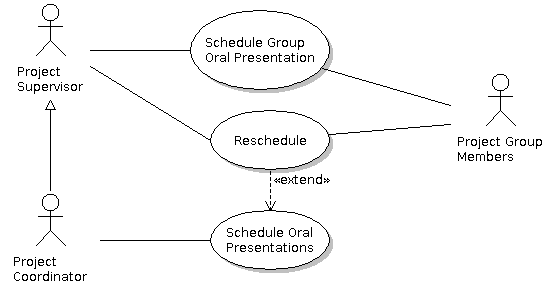
\includegraphics[width=6in]{./img/case-study-fourth-year-system/oral-report-scheduling}
\caption{Use case diagram for the oral presentation functionality of the fourth-year project management system.}
\label{fig:case-4ys-use-case-oral-reports}
\end{figure}


\FloatBarrier

\sectionnote{BM}
\subsection{Project Execution}
\label{sec:4ys-project-execution}

Though all three concerns are important to the system, the most interesting from the point of view of a workflow framework is the project execution phase. This phase accounts for the majority of the lifetime of a fourth-year project, and is also the area in the existing fourth year project management system that could use the most improvement. While account creation and project selection mostly involve basic CRUD (create, read, update, and delete) actions, the execution phase has a well-defined flow:
\begin{enumerate}
\item First, a project proposal must be drafted, submitted, revised, and accepted.
\item After the proposal is accepted, an oral presentation scheduling form must be filled out.
\item Concurrently with scheduling an oral presentation, a progress report must be prepared and submitted.
\item After the progress report is accepted, an oral presentation must be given.
\item After the oral presentation, the group must prepare a presentation for the poster fair. Though this activity has no online deliverables, the group may opt to fill out a poster fair demo request form.
\item While the group is preparing for the poster fair, a final report must also be drafted, submitted, revised, and accepted.
\end{enumerate}
Additionally, each step of the fourth-year project process has associated deadlines.

Use case descriptions for the project execution phase are provided in Tables \ref{tbl:use-case-produce-proposal} through \ref{tbl:use-case-final-report}.

\begin{table}
  \centering
  \caption{Use case description for the ``produce proposal'' use case of the fourth-year project management system.}
  \label{tbl:use-case-produce-proposal}

  \begin{usecase}[Produce Proposal]
    \ucpart{Description}
    Project Group Members produce a project proposal with feedback from their Project Supervisor
    %
    \ucpart{Actors}
    Project Group Member, Project Supervisor
    %
    \ucpart{Preconditions}
    The Project Supervisor has accepted the Project Group Members, but a project proposal has not been completed.
    %
    \ucpart{Flow}
    \ucnormal
    \begin{ucenum}
      \item A Project Group Member uploads and submits a PDF document of the proposal (which for now is a draft.)
      \item The system notifies the Project Supervisor and the other Project Group Members.
      \item The Project Supervisor reviews the proposal draft.
      \item The Project Supervisor provides feedback to the Project Group Members on the proposal draft.
      \item Return to step 1.
    \end{ucenum}
    %
    \ucpart{Variations}
    \ucbranch{A}
    \begin{ucenum}
      \item [A.4] The Project Supervisor accepts the proposal draft.
      \item [A.5] The system marks the draft as the final proposal and notifies the Project Group Members.
    \end{ucenum}
    %
    \ucpart{Exceptions}
    \ucexception{Deadline expires}
    If the proposal is not submitted and finalized before the deadline, it is marked as overdue. The interpretation of this status is left to the Project Supervisor.
    %
    \ucpart{Postconditions}
    A PDF of the proposal is stored and marked as accepted, and project has entered the next phase.
  \end{usecase}
\end{table}


\begin{table}
  \centering
  \caption{Use case description for the ``submit progress report'' use case of the fourth-year project management system.}
  \label{tbl:use-case-submit-progress-report}

  \begin{usecase}[Submit Progress Report]
    \ucpart{Description}
    Project Group Members submit a status update document to their Project Supervisor summarizing their progress on their project.
    %
    \ucpart{Actors}
    Project Group Member, Project Supervisor
    %
    \ucpart{Preconditions}
    The Project Supervisor has accepted a proposal from this group, but has yet to accept a progress report.
    %
    \ucpart{Flow}
    \ucnormal
    \begin{ucenum}
      \item A Project Group Member uploads and submits a PDF document of the progress report.
      \item The system notifies the Project Supervisor and the other Project Group Members.
      \item The Project Supervisor reviews the progress report.
      \item The Project Supervisor accepts the progress report.
    \end{ucenum}
    %
    \ucpart{Variations}
    \ucbranch{A}
    \begin{ucenum}
      \item [A.4] The Project Supervisor returns the progress report.
      \item [A.5] Return to step 1.
    \end{ucenum}
    %
    \ucpart{Exceptions}
    \ucexception{Deadline expires}
    If the progress report is not submitted and finalized before the deadline, it is marked as overdue. The interpretation of this status is left to the Project Supervisor.
    %
    \ucpart{Postconditions}
    A PDF of the progress report is stored, and the project enters the next phase.
  \end{usecase}
\end{table}


\begin{table}
  \centering
  \caption{Use case description for the ``schedule group oral presentation'' use case of the fourth-year project management system.}
  \label{tbl:use-case-schedule-group-oral}

  \begin{usecase}[Schedule Group Oral Presentation]
    \ucpart{Description}
    Project Group Members and their Project Supervisor indicate times that they will be available for the oral presentation.
    %
    \ucpart{Actors}
    Project Group Member, Project Supervisor
    %
    \ucpart{Preconditions}
    The Project Supervisor has accepted a proposal from this group, and the oral presentation scheduling deadline has not passed.
    %
    \ucpart{Flow}
    \ucnormal
    \begin{ucenum}
      \item A Project Group Member fills out the Oral Presentation form.
      \item The system notifies the Project Supervisor and the other Project Group Members.
      \item The Project Supervisor and other Project Group Members review the scheduling form.
      \item The Project Supervisor and all of Project Group Members accept the submitted scheduling form.
      \item The group’s scheduling form is marked is approved.
      \item The oral presentation scheduling deadline expires.
    \end{ucenum}
    %
    \ucpart{Variations}
    \ucbranch{A}
    \begin{ucenum*}
      \item [A.4] Instead of accepting the schedule, a Project Group Member or the Project Supervisor changes the scheduling form.
      \item [A.5] Return to step 2.
    \end{ucenum*}
    \ucbranch{B}
    \begin{ucenum}
      \item [B.6] A Project Group Member or the Project Supervisor changes the scheduling form.
      \item [B.7] Return to step 2.
    \end{ucenum}
    %
    \ucpart{Postconditions}
    The last approved version of the scheduling form is recorded as the scheduling form submitted by the group. If no scheduling form was approved, then a form is submitted with all timeslots marked as available.
  \end{usecase}
\end{table}


\begin{table}
  \centering
  \caption{Use case description for the ``schedule oral presentations'' use case of the fourth-year project management system.}
  \label{tbl:use-case-schedule-orals}

  \begin{usecase}[Schedule Oral Presentations]
    \ucpart{Description}
    The Project Coordinator determines when and where each group will have their oral presentation.
    %
    \ucpart{Actors}
    Project Coordinator
    %
    \ucpart{Preconditions}
    The oral presentation scheduling deadline has passed.
    %
    \ucpart{Flow}
    \ucnormal
    \begin{ucenum}
      \item The Project Coordinator views each groups scheduling form.
      \item The Project Coordinator produces a schedule that best meets the constraints of all of the project groups, assigning each group a time and place for their oral presentation.
      \item The system notifies all Project Group Members and Project Supervisors.
      \item Project Group Members and Project Supervisors view the times and locations of their assigned oral presentations.
    \end{ucenum}
    %
    \ucpart{Exceptions}
    \ucexception{Rescheduling required}
    If a Project Group Member or Project Supervisor is no longer available for the timeslot they were assigned, they must contact the Project Coordinator. The Project Coordinator may choose to repeat the process from step 1 with the new scheduling constraints.
    %
    \ucpart{Postconditions}
    Each group has been assigned an appropriate time and location for their oral presentation.
  \end{usecase}
\end{table}


\begin{table}
  \centering
  \caption{Use case description for the ``submit poster fair demo form'' use case of the fourth-year project management system.}
  \label{tbl:use-case-poster-fair-form}

  \begin{usecase}[Submit Poster Fair Demo Form]
    \ucpart{Description}
    The Project Group Members and Project Supervisor may opt to request space for a demonstration at the poster fair.
    %
    \ucpart{Actors}
    Project Group Members, Project Supervisor
    %
    \ucpart{Preconditions}
    The group’s oral presentation deadline has passed, but the date of the poster fair has not.
    %
    \ucpart{Flow}
    \ucnormal
    \begin{ucenum}
      \item A Project Group Member fills out and submits the poster fair demo request form.
      \item The system notifies the Project Group Members, Project Supervisor, and Project Coordinator.
    \end{ucenum}
    %
    \ucpart{Postconditions}
    The poster fair demo request form has been sent to the Project Coordinator.
  \end{usecase}
\end{table}


\begin{table}
  \centering
  \caption{Use case description for the ``produce final report'' use case of the fourth-year project management system.}
  \label{tbl:use-case-final-report}

  \begin{usecase}[Produce Final Report]
    \ucpart{Description}
    Project Group Members produce a final project report with feedback from their Project Supervisor
    %
    \ucpart{Actors}
    Project Group Member, Project Supervisor, Project Coordinator
    %
    \ucpart{Preconditions}
    The project group has completed their oral presentation, but the final report has not yet been completed. Additionally, the submission deadline for the final report has not passed.
    %
    \ucpart{Flow}
    \ucnormal
    \begin{ucenum}
      \item A Project Group Member uploads and submits a PDF document of the final report (which for now is a draft.)
      \item The system notifies the Project Supervisor and the other Project Group Members.
      \item The Project Supervisor reviews the draft report.
      \item The Project Supervisor provides feedback to the Project Group Members on the draft report.
      \item Return to step 1.
    \end{ucenum}
    %
    \ucpart{Variations}
    \ucbranch{A}
    \begin{ucenum}
      \item [A.4] The Project Supervisor accepts the draft report.
      \item [A.5] The system marks the draft as the final report and notifies the Project Group Members.
      \item [A.6] The system forwards a copy of the final report to the Project Coordinator for distribution to the second reader.
    \end{ucenum}
    %
    \ucpart{Exceptions}
    \ucexception{Deadline expires}
    Submission is closed, and no final report can be submitted after the deadline. If a submission was pending acceptance, it is marked as accepted and proceeds to step A.5.
    %
    \ucpart{Postconditions}
    The project is completed. If the final report was submitted, then the PDF of the final report is stored and marked as accepted, and the Project Coordinator has received a copy.
  \end{usecase}
\end{table}


\FloatBarrier

\sectionnote{AC}
\subsection{Account Management}
\label{sec:account-management}

The account management use cases shown in Figure \ref{fig:case-4ys-use-case-account-management} are described in the following tables \ref{tbl:use-case-create-account} through \ref{tbl:use-case-authenticate}. These descriptions cover the creation, modification, and deletion of the different accounts in the system.


\begin{table}
  \centering
  \caption{Use case description for the ``Create Account'' use case of the fourth-year project management system.}
  \label{tbl:use-case-create-account}

  \begin{usecase}[Create User Account]
    \ucpart{Description}
    Creates a User Account and assign permissions for the newly created User Account
    %
    \ucpart{Actors}
    Project Group Member, Project Coordinator
    %
    \ucpart{Flow}
    \ucnormal
    \begin{ucenum}
      \item The user provides an email address, password, confirmation password, full name, student number, and programme
      \item The system validates and saves the account
    \end{ucenum}
    %
    \ucpart{Exceptions}
    \ucexception{Email not unique}
    An account with that email address already exists and the user is redirected to step 1 and notified of the error
    \ucexception{Password and confirmation password do not match}
    User is redirected to step 1 and notified of the error
    \ucexception{Email address, password, confirmation password, or full name  is not provided}
    User is redirected to step 1 and notified of the error
    %
    \ucpart{Postconditions}
    The User Account is created and saved by the system
  \end{usecase}
\end{table}


\begin{table}
  \centering
  \caption{Use case description for the ``Register Group Member Account'' use case of the fourth-year project management system.}
  \label{tbl:use-case-register-member-account}

  \begin{usecase}[Register Group Member Account]
    \ucpart{Description}
    A student is able to register their own account and their Student Number must be provided and be unique
    %
    \ucpart{Actors}
    Project Group Member
    %
    \ucpart{Description}
    \ucnormal
    \begin{ucenum}
      \item The user provides an email address, password, confirmation password, full name, student number, and programme
      \item The system validates and saves the account, include (Create User Account)
    \end{ucenum}
    %
    \ucpart{Exceptions}
    \ucexception{Student number not unique}
    An account with that student number already exists and the user is redirected to step 1 and notified of the error
    \ucexception{Student number or programme is not provided}
    User is redirected to step 1 and notified of the error
    %
    \ucpart{Postconditions}
    If the Group Member Account was created successfully they will be logged in. If the Group Member Account was not created successfully they will be prompted to attempt to create their account again.
  \end{usecase}
\end{table}


\begin{table}
  \centering
  \caption{Use case description for the ``Manage Account'' use case of the fourth-year project management system.}
  \label{tbl:use-case-manage-account}

  \begin{usecase}[Manage Account]
    \ucpart{Description}
    Any user may edit their own account. Only Project Coordinators are able to edit accounts other than their own.
    %
    \ucpart{Actors}
    Project Group Member, Project Supervisor, Project Coordinator
    %
    \ucpart{Preconditions}
    Account being edited exists
    %
    \ucpart{Flow}
    \ucnormal
    \begin{ucenum}
      \item User provides new account information
      \item The system validates and saves the edited account
    \end{ucenum}
    %
    \ucpart{Variations}
    \ucbranch{A}
    \begin{ucenum}
      \item [A.1] User selects to delete the account
      \item [A.2] The system deletes the account and all references to it
    \end{ucenum}
    %
    \ucpart{Exceptions}
    \ucexception{No privilege to edit\slash delete selected account}
    The account cannot be edited\slash deleted by the current user
    %
    \ucpart{Postconditions}
    If the Account was edited the changes are saved by the system. If the Account was deleted all references to that account and the account itself are removed.
  \end{usecase}
\end{table}


\begin{table}
  \centering
  \caption{Use case description for the ``Authenticate'' use case of the fourth-year project management system.}
  \label{tbl:use-case-authenticate}

  \begin{usecase}[Authenticate]
    \ucpart{Description}
    Authenticate the current User Account
    %
    \ucpart{Actors}
    Project Group Member, Project Supervisor, Project Coordinator
    %
    \ucpart{Preconditions}
    Account being Authenticated exists
    %
    \ucpart{Flow}
    \ucnormal
    \begin{ucenum}
      \item User provides an email address and a password
      \item The system authenticates the user
    \end{ucenum}
    %
    \ucpart{Exceptions}
    \ucexception{Invalid email or password}
    The user is not authenticated and is redirected to step 1 and notified of the error
    %
    \ucpart{Postconditions}
    The User Account was authenticated and is allowed to do any operations that it is allowed.
  \end{usecase}
\end{table}


\FloatBarrier

\sectionnote{BM}
\section{Workflow Design}

With the addition of a ``select  project'' step to account for the project being created and selected in the selection phase, the six-step project execution phase described in section \ref{sec:4ys-project-execution} is the core workflow of a project in the fourth-year project management system. As this high-level workflow is completely linear, it can be trivially transformed into the state chart in Figure \ref{fig:state-machine-project-lifecycle}. In this model, the project is a Stonepath work item, while each step is associated with a set of tasks (ex. producing a proposal or submitting a poster fair demo form), which can be extracted from the use case descriptions in section \ref{sec:4ys-project-execution}.

\begin{figure}[!htbp]
\centering \includegraphics[width=3.8in]{./img/case-study-fourth-year-system/project_lifecycle}
\caption{State chart representation of the workflow for an overall project lifecycle from creation to completion.}
\label{fig:state-machine-project-lifecycle}
\end{figure}

In fact, the majority of the tasks described by the use cases involve the Project Group Members submitting an artifact, the Project Supervisor reviewing it, and then either returning it or accepting it. These tasks can be modelled as Stonepath tasks, which may be assigned to Project Group Members and Project Supervisors. This process is captured in Figure \ref{fig:state-machine-document-submission}. This model leverages Stonepath’s state-based model of tasks to handle multiple activities in parallel (ex. filling out the oral report scheduling form, and producing a progress report.)

\begin{figure}[!htbp]
\centering \includegraphics[width=3.0in]{./img/case-study-fourth-year-system/document_submission}
\caption{State chart representation of a general document submission task, such as proposal submission.}
\label{fig:state-machine-document-submission}
\end{figure}

Other tasks to produce deliverables require only some small modifications to the state chart in Figure \ref{fig:state-machine-document-submission}. For instance, the special handling of deadlines for final reports can easily be handled with two extra state transitions, as Figure \ref{fig:state-machine-final-report-submission} demonstrates. Similarly, the consensus requirement to submit the oral presentation scheduling form only requires a guard clause, while editing a submitted form only requires a new transition back from accepted as demonstrated in Figure \ref{fig:state-machine-oral-presentation-scheduling}.

\begin{figure}[!htbp]
\centering \includegraphics[width=5.5in]{./img/case-study-fourth-year-system/final_report_submission}
\caption{State chart representation of a the final report submission task. This workflow is an extension of the general document submission workflow in Figure \ref{fig:state-machine-document-submission}, with additional transitions for strict handling of missed deadlines.}
\label{fig:state-machine-final-report-submission}
\end{figure}

\begin{figure}[!htbp]
\centering \includegraphics[width=3.5in]{./img/case-study-fourth-year-system/oral_presentation_scheduling}
\caption{State chart representation of a the oral presentation scheduling task. This workflow is an extension of the general document submission workflow in Figure \ref{fig:state-machine-document-submission}, with additional transitions to handle achieving consensus on available times, and to handle editing a submitted form.}
\label{fig:state-machine-oral-presentation-scheduling}
\end{figure}


\FloatBarrier

\sectionnote{BM}
\section{Design}

The design of the system was performed in a top-down fashion, starting from the core project workflow depicted in Figure \ref{fig:state-machine-project-lifecycle}. The system must accommodate multiple concurrent tasks for a user: not only can some states involve multiple tasks, but Project Supervisors may be involved with several project simultaneously. The clearest way to present all of the concurrent tasks for a user is in a tabular view, as depicted in the wireframe in Figure \ref{fig:wireframe-tasks-view}. The user can then select a task from their pending tasks, and carry out the actions associated with its present state.

\begin{figure}[!htbp]
\centering 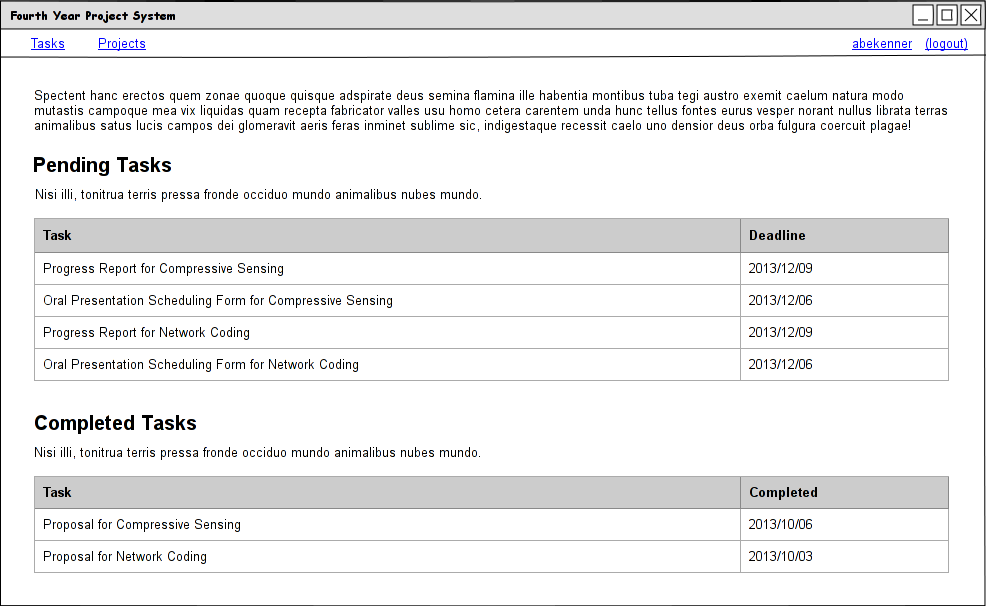
\includegraphics[width=6in]{./img/case-study-fourth-year-system/supervisor-tasks-view_wireframe}
\caption{Wireframe of the tasks view for a Project Supervisor. The tasks view presents the tasks generated by the project state machine in Figure \ref{fig:state-machine-project-lifecycle}. ``Lorem ipsum'' placeholder text has been used in place of introductory and explanatory text.}
\label{fig:wireframe-tasks-view}
\end{figure}

In order to achieve this requirement, the system needs to treat different types of tasks in a project generically - a naive implementation that places each type of task (such as a proposal or progress report) in a discrete ActiveRecord model makes it complex to find all of the outstanding tasks for a user. Stonepath has a SPTask mixin that allows a task to be associated with a workbench (ex. a Project Supervisor) and a workitem (a project). A model extending SPTask might be associated with each task for each workbench / workitem pair, using a polymorphic association. Unfortunately this model is very complex to implement and query, as demonstrated by Figure \ref{fig:sptask-complexity}. Though the relationship between users and tasks is now generic, a polymorphic many-to-many relationship like \verb!Task! is difficult to traverse, as discussed in section \ref{sec:stonepath-prototyping-results}. Additionally, this data model is unnecessarily complex to update in exceptional cases: if a Project Supervisor or Project Group Member needs to be added or removed from the project, then new \verb!Task!s must be added or removed from the database through some means other than the project’s state machine.

\begin{figure}[!htbp]
\centering 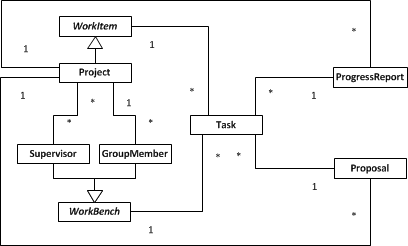
\includegraphics{./img/case-study-fourth-year-system/task-with-sptask-static-structure}
\caption{Logical class diagram of the relationship between concrete tasks of the project workflow (such as proposals and progress reports), projects, supervisors, and group members using Stonepath concepts.}
\label{fig:sptask-complexity}
\end{figure}

Instead of making use of the Stonepath task model, a simpler custom data model was designed instead. As pictured in Figure \ref{fig:custom-task-simplicity}, instances of a new generic \verb!Task! type are associated directly with a project. This is conceptually much simpler, and also allows Project Supervisors and project Group Members to be added and removed from projects without altering the tasks associated with the project.

\begin{figure}[!htbp]
\centering 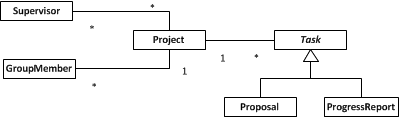
\includegraphics{./img/case-study-fourth-year-system/task-through-project-static-structure}
\caption{Logical class diagram of the relationship between concrete tasks of the project workflow (such as proposals and progress reports), projects, supervisors, and group members using a custom task model.}
\label{fig:custom-task-simplicity}
\end{figure}

With the framework in place to access individual tasks, it was decided that each task in a project would have its own page. In general, task pages are laid out with a detailed task description, followed a short summary of the state of the task, actions that can be performed on the task, and then any other data that is necessary to complete the activity corresponding to the current state of the task. This centralizes information related to a task, and guides the user through the process of completing it. The wireframes in Figures \ref{fig:wireframe-group-member-proposal-view} and \ref{fig:wireframe-supervisor-proposal-view} demonstrate this layout with a proposal task: first, there is a description of the proposal requirements (the task description), followed by a summary of the task state (the file associated with the current submission), actions (``submit'', and ``return'' or ``accept''), and auxiliary data (the submission history.) Note that the actions displayed for the proposal are selected based on the current user's role and the state of the task.

\begin{figure}[!htbp]
\centering 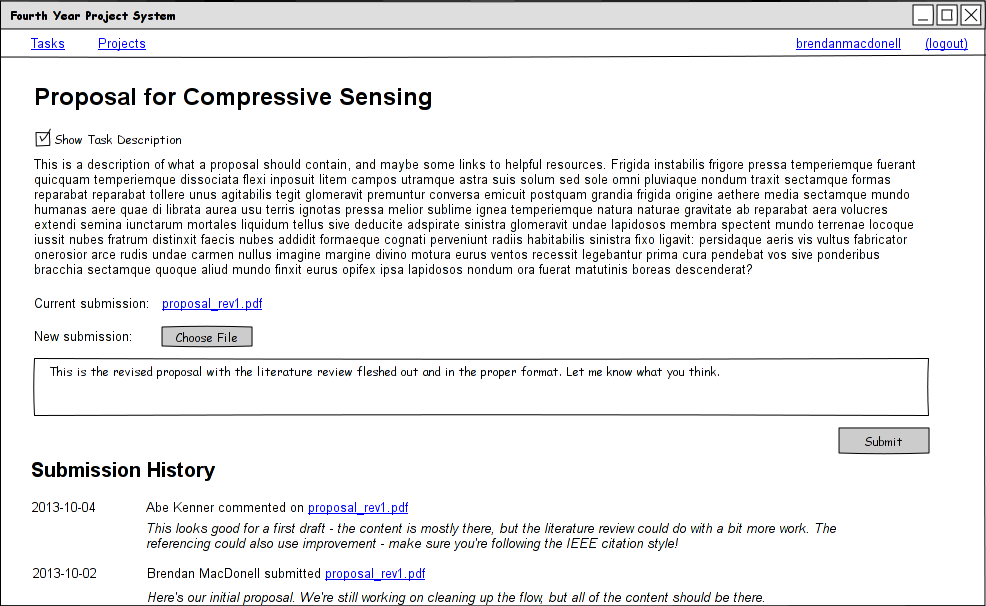
\includegraphics[width=6in]{./img/case-study-fourth-year-system/group-member-proposal-view_wireframe}
\caption{Wireframe of the proposal view of for a Project Group Member when the proposal is in the ``writing submission'' or ``reviewing'' states. The member may upload a new submission with a comment.}
\label{fig:wireframe-group-member-proposal-view}
\end{figure}

\begin{figure}[!htbp]
\centering 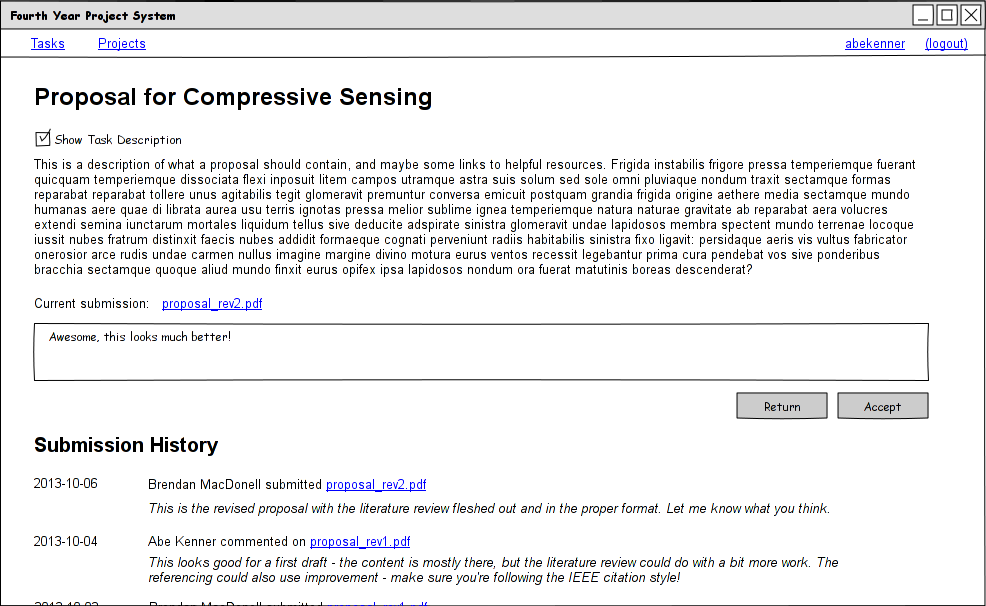
\includegraphics[width=6in]{./img/case-study-fourth-year-system/supervisor-proposal-view_wireframe}
\caption{Wireframe of the proposal view of for a Project Supervisor when the proposal is in the ``reviewing'' state. The supervisor may either return the proposal with a comment, or accept it with a comment.}
\label{fig:wireframe-supervisor-proposal-view}
\end{figure}

Another important feature of the system is user authentication and managing user profile data. From examining the requirements in section \ref{sec:account-management}, it is clear that Project Group Members, Project Supervisors, and Project Coordinators have many profile attributes in common. These attributes are captured in Table \ref{tbl:user-profile-attributes}.

\begin{table}
  \centering
  \caption{User profile attributes used by each role in the system. Note that the attributes for a Group Member are a strict superset of those used by every other role.}
  \label{tbl:user-profile-attributes}
  \tablespacer
  \begin{tabular}{ l l }
    \toprule
    Attribute & Roles \\
    \midrule
    Full name & All \\
    Email & All \\
    Encrypted Password & All \\
    Programme & Project Group Member \\
    Student Number & Project Group Member \\
    Project & Project Group Member \\
    \bottomrule
  \end{tabular}
\end{table}

There are a few ways to model the users, roles, and attributes in the system. One possibility is to represent each role as its own class; however, as Project Coordinators also act as Project Supervisors, this would lead to a confusing ER model, as both classes would need to be related to Tasks and Projects. Additionally, Project Coordinators and Project Supervisors have identical attributes, so this approach would lead to needlessly duplicated code.

A more refined approach would be to model Project Coordinators and Project Supervisors as the same class, with an attribute to discriminate them. This would enable code reuse for the two roles, and would let Project Supervisors become Project Coordinators (and vice versa) without having to delete and recreate their accounts. It would also produce an expressive ER model - Project Coordinators and Project Supervisors could be referenced through the same foreign key, while Project Group Members could not be accidentally associated. Unfortunately, most Account Management use cases in section \ref{sec:account-management} apply to all roles in the system, so separating the role types into distinct classes remains an impediment to code reuse.

The final approach is to combine all of the roles into a single class, and discriminate them based on a role attribute. While this has the disadvantage of producing a less expressive ER model which can’t distinguish references to Supervisors from references to Group Members, it was selected for implementation as it permits significant code reuse for authentication and profile management. Rails has ORM facilities available to ensure that invalid relationships are not saved to the database, which are discussed further in section \ref{sec:4ys-implementation}.

Given a single class to represent a user’s profile, there are two options to represent the user’s role. It could be represented as either a single-valued attribute for simplicity, or a multi-valued attribute to capture the fact that user’s can have multiple effective roles (eg. a Project Coordinator may also fill the role of a Project Supervisor.) However, as only Project Coordinators fill multiple roles, and it is unlikely that the system will develop a need to more granular roles, the decision was made to represent roles as single values and let the implementation handle determining which effective roles a user may fulfill.
